% Newspaper-style feature article (fictional city Marlowe, bike-lane programme). English, 2 pages, two columns.
% Features: masthead, headline and deck, byline, two-column text, pull quote, pgfplots data chart with caption,
% quotes from supporters and critics, a sidebar box with facts.
\documentclass[10pt,a4paper]{article}
\usepackage[T1]{fontenc}
\usepackage[utf8]{inputenc}
\usepackage{mathptmx}
\usepackage[scaled=0.9]{helvet}
\usepackage[english]{babel}
\usepackage[margin=1.7cm,top=1.8cm,bottom=1.9cm]{geometry}
\usepackage{xcolor}
\usepackage{tikz}
\usepackage{pgfplots}
\pgfplotsset{compat=1.18}
\usepackage{multicol}
\usepackage{tcolorbox}
\usepackage{caption}
\usepackage{fancyhdr}
\usepackage{microtype}
\usepackage{enumitem}

\definecolor{ink}{HTML}{1A1A1A}
\definecolor{paperred}{HTML}{9E1B1B}
\setlength{\parindent}{1.1em}
\sloppy
\setlength{\parskip}{0pt}
\setlength{\columnsep}{0.7cm}
\setlength{\columnseprule}{0.3pt}
\captionsetup{font={footnotesize,sf}, labelfont={bf,sf}, labelsep=period, justification=raggedright, singlelinecheck=false}

\pagestyle{fancy}
\fancyhf{}
\renewcommand{\headrulewidth}{0.3pt}
\fancyhead[L]{\sffamily\scriptsize\textbf{THE MARLOWE COURIER}}
\fancyhead[R]{\sffamily\scriptsize Weekend Feature \textperiodcentered{} Saturday, 24 October 2026}
\fancyfoot[C]{\sffamily\scriptsize Fictional newspaper and persons, created for testing purposes only. \hfill \thepage}

\newcommand{\dropquote}[2]{\par\medskip\noindent\begin{tcolorbox}[colback=white, colframe=paperred, boxrule=0pt,
  leftrule=2.5pt, left=7pt, top=3pt, bottom=3pt, sharp corners]
  {\large\itshape #1}\\[2pt]{\sffamily\scriptsize\textbf{#2}}\end{tcolorbox}\medskip}

\begin{document}

% ---- Masthead and headline ------------------------------------------------------------------
\begin{center}
{\Huge\bfseries\textsc{The Marlowe Courier}}\\[-0.1em]
{\sffamily\scriptsize Independent since 1894 \textperiodcentered{} Weekend Feature}
\end{center}
\vspace{-0.4em}\hrule height 1.2pt\vspace{0.12em}\hrule height 0.4pt

\vspace{0.5em}
{\Huge\bfseries Two wheels, one city, a lot of arguments}\par
\vspace{0.3em}
{\Large\itshape Five years and \$152 million into its bike-lane programme, Marlowe has 96 kilometres of
protected lanes, twice as many cyclists on its busiest bridge, and a fierce row about parking.}\par
\vspace{0.4em}
{\sffamily\small By \textbf{Jonas Whitfield}, Transport Correspondent}
\vspace{0.3em}\hrule height 0.4pt\vspace{0.7em}

\begin{multicols}{2}
\raggedcolumns
At 7.40 on a weekday morning, Harbour Bridge belongs to the bicycles. A steady stream of commuters,
students and a few brave delivery riders glides along the separated lane on the downstream side, while
cars queue patiently beside it. Electronic counters on the bridge recorded 6,450 crossings by bicycle on an average
day last year, up from 3,100 in 2020, an increase of 108 percent.

That is the headline result of ``Marlowe Moves'', the cycling programme the city council launched in 2021.
Its goal is a connected network of protected lanes, physically separated from traffic by kerbs, planters
or parked cars. At the end of 2025 the network measured 96 kilometres, up from 18 kilometres five years
earlier. The council wants 140 kilometres by 2028.

\begin{minipage}{\columnwidth}
\centering
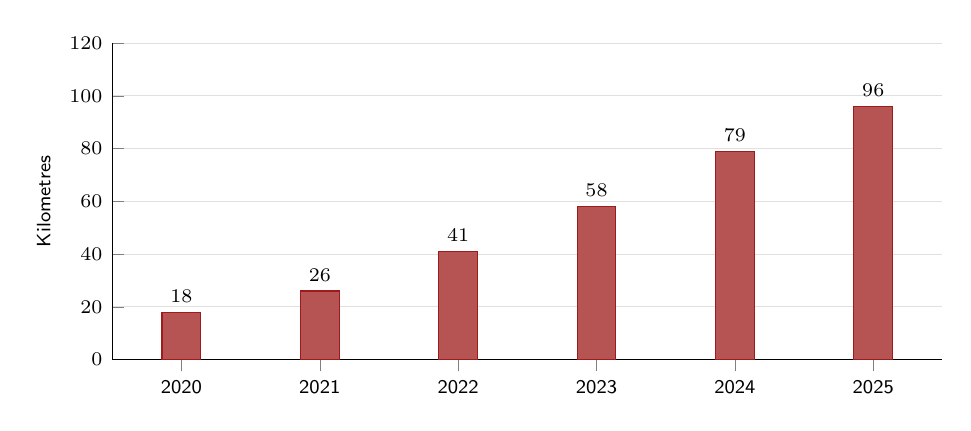
\begin{tikzpicture}
\begin{axis}[
    ybar, bar width=14pt, width=\columnwidth, height=5.6cm,
    ymin=0, ymax=120, ytick={0,20,40,60,80,100,120},
    symbolic x coords={2020,2021,2022,2023,2024,2025}, xtick=data, enlarge x limits=0.1,
    ylabel={Kilometres}, axis x line*=bottom, axis y line*=left, ymajorgrids, grid style={black!12},
    tick label style={font=\sffamily\scriptsize}, label style={font=\sffamily\scriptsize},
    nodes near coords, nodes near coords style={font=\sffamily\scriptsize}]
  \addplot[fill=paperred!75, draw=paperred] coordinates {(2020,18) (2021,26) (2022,41) (2023,58) (2024,79) (2025,96)};
\end{axis}
\end{tikzpicture}
\captionof{figure}{Protected bike lanes in Marlowe at the end of each year, in kilometres. Source: Marlowe Department of Transport.}
\end{minipage}
\medskip


\textbf{More riders, fewer serious injuries.} The share of commuting trips made by bicycle rose from
5.8 percent in 2020 to 10.9 percent in 2025. At the same time, the number of seriously injured cyclists
reported to the police fell from 112 to 74 a year, a drop of 34 percent. ``Separated lanes work because they
remove the conflict,'' says Dr.\ Samuel Reyes, a transport researcher at Marlowe University. ``Most serious
injuries happen at junctions and when cars overtake closely. A kerb solves the second problem entirely.''

\dropquote{``My children ride to school alone now. Five years ago I would not have let them.''}{Tomas Ellery, father of two, Eastfield}

Supporters point to a public opinion survey of 1,200 residents carried out in spring 2026: 63 percent of
respondents support the programme, 29 percent oppose it and 8 percent are undecided. Priya Nandakumar, chair
of the council's transport committee, says the figures show a majority that is ``tired of being told this city
is built for cars.'' She argues that every lane kilometre is cheaper than a kilometre of road widening.


\textbf{The price of progress.} Not everyone is convinced. To make room for the lanes, the city has removed
1,340 on-street parking spaces, about 9 percent of the total in the centre. Walter Brandt, chairman of the
Downtown Merchants Association, calls the cost ``far higher than the council admits.'' A survey of his members
found that 31 percent of shops on streets with new lanes reported lower sales, 24 percent reported higher
sales and 45 percent saw no change.

\dropquote{``A bakery lives from people who stop for two minutes. If they cannot park, they go to the supermarket.''}{Linnea Okafor, owner of Okafor's Bakery, Harbour Street}

Researchers are cautious about such claims. Dr.\ Reyes notes that studies in other cities usually find that
shops on cycle-friendly streets do at least as well as before, ``but a bakery that depends on short car trips
may genuinely be an exception.'' The council has promised a loading-zone rule for deliveries and a study of
sales figures, to be published next spring.

Money is the second line of attack. The programme has a budget of \$214 million up to 2028, of which \$152
million has been spent. That works out at roughly \$1.6 million per kilometre of lane, with the most
complex junctions costing several times the average. Critics in the opposition group also say the lanes
are unevenly spread: the western districts have 71 kilometres, the poorer eastern districts only 25.

\textbf{A tale of two districts.} The geography of the network is the sharpest political issue. The
western districts, with their wealthier households and shorter distances to the centre, have 71 kilometres
of protected lanes; the eastern districts, where the bus network is thinner and car ownership lower, have
25. Marcus Hale, who leads the opposition on the council, says the money has been spent ``where the votes
are, not where the need is.'' Ingrid Solberg, director of the cycling group Pedal Marlowe and an
outspoken supporter of the programme, agrees on that point, if on little else. ``Phase 3 must go east
first,'' she says.

The council has taken the criticism on board. Of the 44 kilometres planned for Phase 3, 29 will be built in
the eastern districts and 15 in the west. That would bring the two halves of the city to 54 and 86
kilometres respectively.

\textbf{How Marlowe compares.} With about 410,000 residents, Marlowe has 23 kilometres of protected lanes
per 100,000 inhabitants. That puts it fifth among twelve mid-sized cities in the national cycling
ranking. The leader, Kestrel, has 41 kilometres per 100,000. Dr.\ Reyes warns against reading too much into
league tables. ``Kilometres are easy to count,'' he says. ``What matters is whether the lanes connect, and
Marlowe still has gaps, above all around the central station.''

\textbf{What comes next.} Phase 3 will add another 44 kilometres, including long-awaited lanes on Mill Road
and Harbour Street, and bring the network to the target of 140 kilometres by 2028. The detailed plans go
out for public consultation until 30 November 2026. ``We will not please everyone,'' says Ms Nandakumar. ``But
we have a better idea now of what works, and we will use it.''

\begin{tcolorbox}[colback=black!5, colframe=ink, boxrule=0.5pt, sharp corners, left=6pt, right=6pt, top=4pt, bottom=4pt,
  title={\sffamily\bfseries Marlowe Moves at a glance}, fonttitle=\sffamily\small, coltitle=white, colbacktitle=ink]
\sffamily\footnotesize
\begin{itemize}[leftmargin=1.0em, itemsep=1pt, topsep=1pt]
  \item \textbf{Launched:} 2021
  \item \textbf{Budget to 2028:} \$214 million (\$152 million spent)
  \item \textbf{Protected lanes:} 96 km (2025), target 140 km (2028)
  \item \textbf{Phase 3:} 44 km, including Mill Road and Harbour Street
  \item \textbf{Bike share of commuting:} 10.9 percent (2020: 5.8 percent)
  \item \textbf{Seriously injured cyclists:} 74 a year (2020: 112)
  \item \textbf{Parking spaces removed:} 1,340
  \item \textbf{Have your say:} consultation open until 30 November 2026 at marlowe.example/moves
\end{itemize}
\end{tcolorbox}
\end{multicols}

\end{document}
